\documentclass[11pt,paper=a4,footinclude=true,headinclude=true,open=any]{scrbook}
\usepackage[T1]{fontenc}
\usepackage[utf8]{inputenc}
\usepackage[parts=false,eulerchapternumbers]{classicthesis}

% ---------------------------------------------------------------------
% Palette: four custom colours, then re-skin classicthesis' own
% internal named colours so links, citations and chapter numerals
% follow the same palette instead of the package defaults.
% ---------------------------------------------------------------------
\definecolor{claybrick}{RGB}{150,58,42}
\definecolor{slatestone}{RGB}{54,70,82}
\definecolor{parchment}{RGB}{247,242,232}
\definecolor{umberink}{RGB}{40,34,29}

\definecolor{CTtitle}{RGB}{150,58,42}
\definecolor{CTlink}{RGB}{54,70,82}
\definecolor{CTurl}{RGB}{54,70,82}
\definecolor{CTcitation}{RGB}{54,70,82}
\definecolor{CTsemi}{RGB}{178,170,160}

\usepackage{amsmath}
\usepackage{amssymb}
\usepackage{epigraph}
\usepackage{tikz}
\usepackage{tcolorbox}

\setlength{\epigraphwidth}{0.62\textwidth}
\renewcommand{\epigraphflush}{flushright}
\setlength{\epigraphrule}{0pt}

\tcbset{
  colframe=slatestone,
  colback=parchment,
  colbacktitle=slatestone,
  coltitle=parchment,
  fonttitle=\spacedlowsmallcaps,
  boxrule=0.5pt,
  arc=0pt,
  left=8pt,right=8pt,top=5pt,bottom=5pt
}

\begin{document}

\frontmatter

\begin{titlepage}
\thispagestyle{empty}
\begin{flushright}
\vspace*{3.6cm}
{\fontsize{30}{36}\selectfont\color{umberink}\spacedallcaps{The Quiet Page}}\par
\vspace{0.7cm}
{\Large\itshape\color{claybrick}Order, Proportion, and the\\ Architecture of the Scholarly Book}\par
\vspace{2.4cm}
{\large\spacedlowsmallcaps{Anneke Voss}}\par
\vspace{0.35cm}
{\small\color{slatestone}\spacedlowsmallcaps{Department of Book Arts and Typography}\\
\spacedlowsmallcaps{Meridian University}}\par
\vspace*{\stretch{1}}
\begin{tikzpicture}
\draw[claybrick,line width=0.6pt] (0,0) -- (4.2,0);
\end{tikzpicture}\par
\vspace{0.3cm}
{\small\color{umberink}First Edition --- \the\year}
\end{flushright}
\end{titlepage}

\tableofcontents

\mainmatter
\pagestyle{scrheadings}

\chapter{The Problem of the Page}
\label{chap:problem}

\epigraph{A page that announces its own structure has already failed it.}{---\textsc{Ilse Ferrer}, \emph{Silent Grids}}

Every printed page makes an argument before a single word of its text is read. The width of its margins, the darkness of its type, the interval between one line and the next: these are decisions, not accidents, and a reader who cannot name them is nonetheless governed by them. This treatise concerns the small number of proportions and intervals that, taken together, allow a page of continuous prose to be read for an hour without the reader once becoming aware of the page itself.

That invisibility is the discipline's oldest and least fashionable ambition. It is easy to design a page that is noticed; it is difficult to design one that is not. The chapter that follows treats two such quiet mechanisms in turn -- the geometry by which a text block is set into its sheet, and the grammar by which a paragraph's measure and leading are chosen -- before closing with a word on restraint (Chapter~\ref{chap:geometry}).

None of it is new. The canon of proportion was already old when the first printed books adopted it from manuscript practice, and the measure-and-leading relationships have been rediscovered, independently, by nearly every generation of book designers since. What follows is not novelty but an account of \emph{why} these conventions persist: not out of habit, but because each solves a specific, recurring problem of the reading eye.

\chapter{The Geometry of the Page}
\label{chap:geometry}

\epigraph{The margin is not empty. It is where the hand rests.}{---\textsc{Anneke Voss}, field notes, 2019}

\section{A Canon of Page Construction}
\label{sec:canon}

Before a single line of type is set, the page has already been divided. A sheet of paper of ratio $2:3$ -- close to the proportion of a folio leaf since the earliest bound books -- can be partitioned by a construction as old as it is elegant: the diagonals of the leaf are drawn, and the point at which they cross, together with a diagonal drawn from a single corner, fixes the inner corner of the text block. The resulting block is geometrically similar to the page that contains it, and its margins fall, without further calculation, into a hierarchy every practised eye recognises as correct: spine narrowest, head next, fore-edge wider still, tail widest of all.

\begin{figure}[h]
\centering
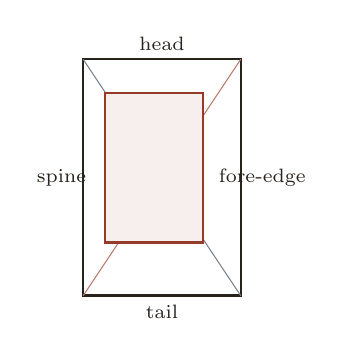
\begin{tikzpicture}[scale=0.5]
  \coordinate (A) at (0,0);
  \coordinate (B) at (4,0);
  \coordinate (C) at (4,6);
  \coordinate (D) at (0,6);
  \draw[umberink,thick] (A) rectangle (C);
  \draw[claybrick!65,thin] (A) -- (C);
  \draw[slatestone!65,thin] (B) -- (D);
  \coordinate (E) at (0.55,1.35);
  \coordinate (F) at (3.05,1.35);
  \coordinate (G) at (3.05,5.15);
  \coordinate (H) at (0.55,5.15);
  \draw[claybrick,thick,fill=claybrick!8] (E) rectangle (G);
  \node[font=\scriptsize,color=umberink] at (-0.55,3) {spine};
  \node[font=\scriptsize,color=umberink] at (4.55,3) {fore-edge};
  \node[font=\scriptsize,color=umberink] at (2,6.4) {head};
  \node[font=\scriptsize,color=umberink] at (2,-0.4) {tail};
\end{tikzpicture}
\caption{The classical diagonal construction, shown on a single leaf. The crossing diagonals fix the inner corner of the text block; the block shares the leaf's proportion and inherits its narrow-to-wide margin sequence: spine, head, fore-edge, tail.}
\label{fig:canon}
\end{figure}

The hierarchy is not decorative. A spine margin must be narrow because the gutter itself, once bound, already swallows a portion of it; a tail margin must be wide because a hand holding an open book rests along the bottom edge, and because the eye, dropping from the last line of a page, needs a visible place to stop. Ferrer's survey of surviving fifteenth-century bindings found the same hierarchy in volumes that could not have shared a workshop -- evidence, in her phrase, that it is ``a solution the material keeps insisting on.''

A designer who instead centres the text block -- equal margins on all sides -- produces a page that photographs well and reads badly: the block appears to slide downward, because the eye judges vertical position by the weight below a shape, not by the ruled distance to its edge. The unequal canon corrects an optical illusion that an equal margin would otherwise leave uncorrected.

\section{Measure, Grid, and the Grammar of the Paragraph}
\label{sec:measure}

Once a text block is fixed, it must be filled, and here a second proportion governs: the relationship between a line's length -- its \emph{measure} -- and the space between one baseline and the next -- its \emph{leading}. Neither can be chosen without the other. A wide measure read at single-line spacing forces the eye to hunt for the start of the next line and, missing it, to re-read the line just finished; a narrow measure read at generous leading produces a page so pale and broken that no rhythm of reading can establish itself at all.

The rule of thumb -- prescribed independently by nearly every manual of book typography since the interwar period -- holds that a measure should carry fifty to seventy-five lowercase characters, including spaces, with leading expanding as the measure approaches the upper end of that range. Table~\ref{tab:specimens} gives four representative text faces set to this discipline.

\begin{table}[h]
\centering
\small
\begin{tabular}{@{}lccc@{}}
\toprule
Typeface & Rel.\ x-height & Measure (cpl) & Leading ($\times$ size) \\
\midrule
Solenne Text & 0.47 & 62--68 & 1.20 \\
Corvina Old Style & 0.44 & 58--64 & 1.15 \\
Alden Serif & 0.52 & 66--72 & 1.30 \\
Marchetti Antiqua & 0.49 & 60--66 & 1.22 \\
\bottomrule
\end{tabular}
\caption{Recommended measure and leading for four representative book text faces, each set at 10.5\,pt body size.}
\label{tab:specimens}
\end{table}

A face with a large relative x-height -- Alden Serif, above -- reads comfortably at a wider measure, because its lowercase letters present more distinguishing shape at a given size; a smaller x-height, as in Corvina Old Style, needs a narrower column to keep the eye's return sweep accurate.

\begingroup
\small
\begin{tcolorbox}[title=Editorial Note]
Halvorsen's 2019 reading-comfort trials found comprehension losses at both extremes of the fifty-to-seventy-five range, but the \emph{location} of the comfortable middle moved by nearly eight characters between the widest- and narrowest-set faces tested. Table~\ref{tab:specimens} is a starting hypothesis for a given face, to be confirmed by proofing -- not a substitute for it.
\end{tcolorbox}
\endgroup

The golden section is sometimes invoked as a further constraint, and it is worth stating precisely what it does and does not license:
\[
\varphi = \frac{1+\sqrt{5}}{2} \approx 1.618.
\]
A text block whose height-to-width ratio approximates $\varphi$ tends to look settled rather than arbitrary. But $\varphi$ constrains only the \emph{shape} of a rectangle; a page can be golden in proportion and still unreadable in its type.

\section{Toward a Typography of Restraint}
\label{sec:conclusion}

The proportions gathered here share one character: none is visible, as such, to a reader doing what a reader does, which is to forget the page and attend to the sentence. A designer who wishes to be noticed will always find room to depart from them; a designer who wishes to be read will find, more often than not, that the departure was not necessary.

Voss's own working rule is a fitting close: a page is finished not when nothing more can be added to it, but when nothing more can be taken away without the reader noticing the loss.

\backmatter

\begin{thebibliography}{9}
\bibitem{voss2021}
Voss, A. (2021). \emph{The Quiet Page: Studies in Book Proportion}. Meridian University Press.

\bibitem{ferrer2018}
Ferrer, I. (2018). \emph{Silent Grids: Structure in the Renaissance Page}. Nimbus Editions.

\bibitem{halvorsen2019}
Halvorsen, K. (2019). \emph{Measure and Memory: Reading Comfort in Long-Form Text}. Apex Scholarly Press.

\bibitem{doyle2015}
Doyle, M. (2015). \emph{The Grammar of the Grid}. Vertex Editions.

\bibitem{marchetti2012}
Marchetti, S. (2012). \emph{Type on Paper: A Working Anatomy}. Synapse House.

\end{thebibliography}

\end{document}
